    %-------------------------
% Resume in Latex
% Author
% License : MIT
%------------------------

%---- Required Packages and Functions ----

\documentclass[a4paper,11pt]{article}
\usepackage{latexsym}
\usepackage{xcolor}
\usepackage{float}
\usepackage{ragged2e}
\usepackage[empty]{fullpage}
\usepackage{wrapfig}
\usepackage{lipsum}
\usepackage{tabularx}
\usepackage{titlesec}
\usepackage{geometry}
\usepackage{marvosym}
\usepackage{verbatim}
\usepackage{enumitem}
\usepackage[hidelinks]{hyperref}
\usepackage{fancyhdr}
\usepackage{fontawesome5}
\usepackage{multicol}
\usepackage{graphicx}
\usepackage{cfr-lm}
\usepackage[T1]{fontenc}
\setlength{\multicolsep}{0pt} 
\pagestyle{fancy}
\fancyhf{} % clear all header and footer fields
\fancyfoot{}
\renewcommand{\headrulewidth}{0pt}
\renewcommand{\footrulewidth}{0pt}
\geometry{left=1.4cm, top=0.8cm, right=1.2cm, bottom=1cm}
% Adjust margins
%\addtolength{\oddsidemargin}{-0.5in}
%\addtolength{\evensidemargin}{-0.5in}
%\addtolength{\textwidth}{1in}
\usepackage[most]{tcolorbox}
\tcbset{
	frame code={}
	center title,
	left=0pt,
	right=0pt,
	top=0pt,
	bottom=0pt,
	colback=gray!20,
	colframe=white,
	width=\dimexpr\textwidth\relax,
	enlarge left by=-2mm,
	boxsep=4pt,
	arc=0pt,outer arc=0pt,
}

\urlstyle{same}

\raggedright
\setlength{\tabcolsep}{0in}


% Sections formatting
\titleformat{\section}{
  \vspace{-4pt}\scshape\raggedright\large
}{}{0em}{}[\color{black}\titlerule \vspace{-7pt}]

%-------------------------
% Custom commands
\newcommand{\resumeItem}[2]{
  \item{
    \textbf{#1}{\hspace{0.5mm}#2 \vspace{-0.5mm}}
  }
}

\newcommand{\resumePOR}[3]{
\vspace{0.5mm}\item
    \begin{tabular*}{0.97\textwidth}[t]{l@{\extracolsep{\fill}}r}
        \textbf{#1}\hspace{0.3mm}#2 & \textit{\small{#3}} 
    \end{tabular*}
    \vspace{-2mm}
}

\newcommand{\resumeSubheading}[4]{
\vspace{0.5mm}\item
    \begin{tabular*}{0.98\textwidth}[t]{l@{\extracolsep{\fill}}r}
        \textbf{#1} & \textit{\footnotesize{#4}} \\
        \textit{\footnotesize{#3}} &  \footnotesize{#2}\\
    \end{tabular*}
    \vspace{-2.4mm}
}

\newcommand{\resumeProject}[4]{
\vspace{0.5mm}\item
    \begin{tabular*}{0.98\textwidth}[t]{l@{\extracolsep{\fill}}r}
        \textbf{#1} & \textit{\footnotesize{#3}} \\
        \footnotesize{\textit{#2}} & \footnotesize{#4}
    \end{tabular*}
    \vspace{-2.4mm}
}

\newcommand{\resumeSubItem}[2]{\resumeItem{#1}{#2}\vspace{-4pt}}
% \renewcommand{\labelitemii}{$\circ$}
\renewcommand{\labelitemi}{$\vcenter{\hbox{\tiny$\bullet$}}$}
\newcommand{\resumeSubHeadingListStart}{\begin{itemize}[leftmargin=*,labelsep=0mm]}
\newcommand{\resumeHeadingSkillStart}{\begin{itemize}[leftmargin=*,itemsep=1.7mm, rightmargin=2ex]}
\newcommand{\resumeItemListStart}{\begin{justify}\begin{itemize}[leftmargin=3ex, rightmargin=2ex, noitemsep,labelsep=1.2mm,itemsep=0mm]\small}
\newcommand{\resumeSubHeadingListEnd}{\end{itemize}\vspace{2mm}}
\newcommand{\resumeHeadingSkillEnd}{\end{itemize}\vspace{-2mm}}
\newcommand{\resumeItemListEnd}{\end{itemize}\end{justify}\vspace{-2mm}}
\newcommand{\cvsection}[1]{%
\vspace{2mm}
\begin{tcolorbox}
    \textbf{\large #1}
\end{tcolorbox}
    \vspace{-4mm}
}
\newcolumntype{L}{>{\raggedright\arraybackslash}X}%
\newcolumntype{R}{>{\raggedleft\arraybackslash}X}%
\newcolumntype{C}{>{\centering\arraybackslash}X}%
%---- End of Packages and Functions ------

%-------------------------------------------
%%%%%%  CV STARTS HERE  %%%%%%%%%%%
%%%%%% DEFINE ELEMENTS HERE %%%%%%%
\newcommand{\name}{Agus Fuad Mudhofar} % Your Name
\newcommand{\course}{Computer Engineering} % Your Program
% \newcommand{\roll}{xxxxxxx} % Your Roll No.
\newcommand{\phone}{8882111890} % Your Phone Number
\newcommand{\emaila}{agusfuad090@gmail.com} %Email 1

\begin{document}
\fontfamily{cmr}\selectfont
%----------HEADING-----------------
{
  \noindent
\begin{tabularx}{\linewidth}{@{} l L r @{}}
    % Foto
    \raisebox{-0.5\height}{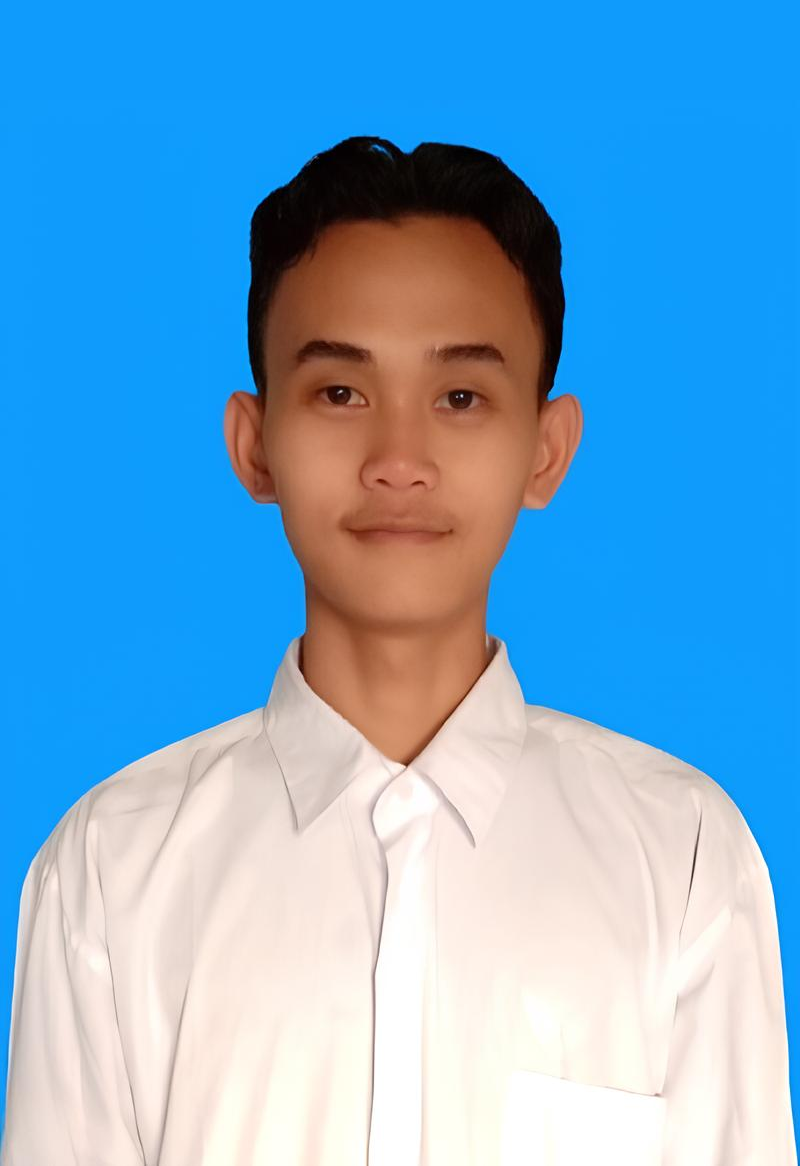
\includegraphics[width=2.5cm]{PAS FOTO Upscale.png}}\hspace{0.5cm} &
    
    % Nama & institusi
    \begin{tabular}[t]{@{}l@{}}
        \textbf{\Large \name} \\
        Institut Teknologi Sepuluh Nopember \\
        Surabaya, Indonesia
    \end{tabular}
    &
    
    % Kontak
    \begin{tabular}[t]{@{}r@{}}
        \raisebox{0.0\height}{\footnotesize \faPhone}\ +62-\phone \\
        \href{mailto:\emaila}{\raisebox{0.0\height}{\footnotesize \faEnvelope}\ \emaila} \\
        \href{https://maedakenji.github.io/Portofolio/}{\raisebox{0.0\height}{\footnotesize \faGithub}\ GitHub} \\
        \href{https://www.linkedin.com/in/agus4434/}{\raisebox{0.0\height}{\footnotesize \faLinkedin}\ LinkedIn}
    \end{tabular}
\end{tabularx}

}

% ------------Personal Details----------------
\section{\textbf{Personal Details}}
NIK: 3207202108040005 \\
NIM: 5024221021


%-----------EDUCATION-----------
\section{\textbf{Education}}
\resumeSubHeadingListStart
\resumeSubheading
{Bachelor of Computer Engineering}{GPA: 3.64}
{Institut Teknologi Sepuluh Nopember, Surabaya}{2022-Present}
\resumeSubHeadingListEnd
\vspace{-5.5mm}
%

%-----------PROJECTS-----------------
\section{\textbf{Personal Projects}}
\resumeSubHeadingListStart

\resumeProject
{Smart Wheelchair with Eye Movement Control} % Project Name
{A smart wheelchair system controlled by eye movement, integrating computer vision and embedded hardware.} % Project Description
{} % Event Dates

\resumeItemListStart
\item {Developed a smart wheelchair system that allows users to control movement using eye gaze, enhancing accessibility for individuals with mobility impairments.}
\item {Integrated real-time eye tracking and gesture recognition using Python and OpenCV, enabling intuitive navigation and control.}
\item {Implemented embedded hardware components (Arduino/ESP32) for motor control and sensor feedback, ensuring reliable operation.}
\item {Collaborated with a team to design, prototype, and test the system, resulting in a functional prototype showcased at the GEMASTIK XVII competition.}
\item {Technology Used: Python, OpenCV, Arduino/ESP32, C/C++, computer vision algorithms.}
\resumeItemListEnd
\vspace{-2mm}

\resumeProject
{Sappy: Multi-Role Livestock Management App (Flutter)} % Project Name
{A livestock management app for multiple roles (Farmer, Admin, Doctor) with NFC support.}
{} % Event Dates

\resumeItemListStart
\item {Provides role-based access and dashboards for farmers, administrators, and doctors, all in a unified mobile app.}
\item {Supports English and Indonesian languages using built-in localization.}
\item {Implements state management via Provider and enables NFC functionality for secure identification and tracking.}
\item {Includes data visualization, authentication, and environmental configuration using modern Flutter ecosystem packages.}
\item {Technology Used: Flutter, Dart, Provider, NFC, fl\_chart, carousel\_slider, custom fonts/assets.}
\resumeItemListEnd
\vspace{-2mm}

\resumeProject
{Comic Reading Web Application} % Project Name
{A web-based comic reading platform supporting manga, manhua, and manhwa with optimized reading experience.} % Project Description
{} % Event Dates
{}
\resumeItemListStart
\item {Developed a responsive comic reading platform supporting manga, manhua, and manhwa with smooth page navigation and optimized image rendering.}
\item {Implemented core reading features including chapter management, reading history, authentication, and adaptive layouts for multiple devices.}
\item {Technology Used: React (frontend), Laravel (backend/API), PostgreSQL (database), with modular component architecture and optimized asset handling.}
\resumeItemListEnd
\vspace{-2mm}

% ---------------End of Projects
\resumeSubHeadingListEnd
\vspace{-4mm}

% %-----------EXPERIENCE-----------------
\section{\textbf{Experience}}
\resumeSubHeadingListStart
% Start of Experience 1
\resumeSubheading
{Web Developer – MIOT Webpage}
{Multimedia and IoT Laboratory (MIOT)}
{Surabaya}{Aug 2024- Present}
\resumeItemListStart
\item {Designed and developed the official MIOT laboratory webpage to showcase research, publications, and team members.}
\item {Implemented a responsive and modern user interface using React.js and Tailwind CSS, ensuring accessibility across devices.}
\item {Integrated dynamic content management for news, events, and member profiles using JSON-based data structures.}
\item {Collaborated with lab members to gather requirements, iterate on design, and deploy the site using GitHub Pages.}
\item {Optimized site performance and SEO, and provided documentation for future maintenance and updates.}
\resumeItemListEnd
\vspace{-4mm}

\clearpage
\resumeSubheading
{Research Assistant – Multimedia and IoT Lab (B300)}{Multimedia and IoT Laboratory (MIOT)}
{Surabaya}{April - June 2025}
\resumeItemListStart
\item {Conducted research on deploying deep learning models on edge devices using NVIDIA Jetson Nano, focusing on computer vision tasks.}
\item {Developed and optimized object detection pipelines using Python and C++ with MobileNet-SSD, YOLOv5n, and YOLOv11s architectures.}
\item {Explored model conversion and acceleration techniques with ONNX and NVIDIA TensorRT for real-time inference.}
\item {Integrated and evaluated models within the NVIDIA DeepStream SDK for efficient video analytics and deployment.}
\item {Benchmarked performance and resource utilization to optimize inference speed and accuracy in constrained environments.}
\resumeItemListEnd
\vspace{-2mm}

\resumeSubheading
{Lab Teaching Assistant – Basic Programming}{Multimedia and IoT Laboratory (MIOT)}
{Surabaya}{Aug 2025 - Nov 2025}
\resumeItemListStart
\item {Developed and maintained lab materials, including coding exercises and troubleshooting guides during practicum, while also being responsible for deploying and maintaining the DMOJ online judge website used in coursework.}
\item {Guided students through practical assignments in C/C++, providing real-time support and technical explanations.}
\item {Evaluated student submissions, provided constructive feedback, and contributed to grading rubrics to ensure fair and consistent assessment.}
\item {Organized and led review sessions before exams, addressing common misconceptions and reinforcing key programming concepts.}
\resumeItemListEnd
\vspace{-2mm}

\resumeSubheading
{Lab Teaching Assistant – Digital Systems}{Robotics and Digital Systems Laboratory (B401)}
{Surabaya}{Mar 2025 - May 2025}
\resumeItemListStart
\item {Conducted lab sessions for \textit{Rangkaian Digital}, supporting over 100 undergraduate students each semester.}
\item {Developed and maintained lab materials, including hardware schematics and troubleshooting guides for digital logic experiments.}
\item {Guided students through practical assignments in digital circuit design, providing real-time support and technical explanations.}
\item {Collaborated with faculty to improve lab workflows, implement new teaching tools, and enhance the overall learning experience.}
\item {Organized and led review sessions before exams, addressing common misconceptions and reinforcing key concepts in digital systems.}
\resumeItemListEnd
\vspace{-2mm}

\resumeSubheading
{Lab Teaching Assistant – Telemathics Workshop}{Robotics and Digital Systems Laboratory (B401)}
{Surabaya}{Mar 2025 - May 2025}
\resumeItemListStart
\item {Prepared and developed practicum modules and instructional materials for \textit{Workshop Telematika}, ensuring structured, hands-on learning for undergraduate students.}
\item {Supervised and guided students during laboratory sessions, particularly in hardware-oriented activities including manual soldering, 3D design for prototyping, hot air rework (blower) soldering,  reflow soldering, and 3D printing.}
\item {Provided real-time technical assistance in C/C++ programming and microcontroller-based experiments, helping students troubleshoot both software and hardware issues.}
\item {Assessed student practicum results, delivered constructive feedback, and contributed to grading criteria to ensure fair and consistent evaluation.}
\item {Organized and led review sessions prior to assessments, reinforcing key concepts and practical skills.}
\resumeItemListEnd

\resumeSubHeadingListEnd
\vspace{-5.5mm}
\section{\textbf{Positions of Responsibility}}
\resumeSubHeadingListStart
\resumeSubheading
{Team Leader – GEMASTIK XVII (IoT Division)}
{Semarang State University (UNNES)}{Semarang}
% {Sambal Telur Team (ITS)}
% {Semarang State University (UNNES)}
{Jan - Nov 2024}

\resumeItemListStart
\item {Led a team representing Institut Teknologi Sepuluh Nopember in the Smart Devices, Embedded Systems, and IoT Division at GEMASTIK XVII.}
\item {Coordinated the team’s efforts across software and hardware components, managed timelines, and delegated responsibilities.}
\item {Developed a smart wheelchair system controllable via eye movement, integrating computer vision and embedded hardware.}
\item {Secured the National Finalist award (Juara Harapan) through efficient planning, ideation, and execution of an IoT-based innovation.}
\resumeItemListEnd
\vspace{-4mm}

\resumeSubheading
{Workshop Assistant – International Workshop on Deep Learning}
{Institut Teknologi Sepuluh Nopember}{Surabaya}
{24 - 29 Nov 2025}

\resumeItemListStart
\item {Assisted in the execution of a 5-day international workshop focused on machine learning and deep learning applications for assistive technology.}
\item {Provided hands-on support to participants by helping resolve technical issues and learning difficulties during workshop sessions.}
\item {Supported professors and speakers in running the event, including administrative coordination and on-site logistical tasks.}
\item {Contributed to creating an inclusive and supportive learning environment for students from Malaysia, Vietnam, the Philippines, Ethiopia, Pakistan, and Indonesia.}
\resumeItemListEnd

\clearpage
\resumeSubheading
{Head of Logistics Department – Multimedia and Game Event (MAGE X)}
{Multimedia and Game Event (MAGE X)}
{Surabaya}{Jan - November 2024}
\resumeItemListStart
\item {Led the logistics team for MAGE X, a major university-level multimedia and game competition event.}
\item {Coordinated procurement, inventory management, and distribution of event materials and equipment.}
\item {Developed and executed logistics plans to ensure timely setup and smooth operation across multiple event venues.}
\item {Collaborated with other departments to address real-time needs and resolve logistical challenges during the event.}
\item {Managed vendor relations, budget tracking, and post-event inventory reconciliation.}
\resumeItemListEnd
\vspace{-4mm}
\resumeSubHeadingListEnd

\section{\textbf{Organizational Experience}}
\resumeSubHeadingListStart
\resumeSubheading
{Member – Multimedia and IoT Laboratory (MIOT)}
{Institut Teknologi Sepuluh Nopember}{Surabaya}{2025 - Present}
\resumeItemListStart
\item {Participated in research projects focused on multimedia systems, IoT applications, and embedded systems.}
\item {Contributed to lab activities, including seminars, workshops, and collaborative research initiatives.}
\item {Engaged in knowledge-sharing sessions and technical discussions with lab members and faculty.}
\resumeItemListEnd

\resumeSubheading
{Member – UKM Rebana ITS}
{Institut Teknologi Sepuluh Nopember}{Surabaya}{2022 - 2023}
\resumeItemListStart
\item {Active member of the university's traditional music ensemble, specializing in Rebana performances.}
\item {Participated in various cultural events and showcasing traditional music and promoting cultural heritage.}
\item {Collaborated with fellow members to organize rehearsals, performances, and community outreach activities.}
\item {Project Leader for Welcome Party 2022; organized events to welcome and integrate incoming students into UKM Rebana ITS.}
\resumeItemListEnd

\resumeSubheading
{Expert Staff – UKM Rebana ITS}
{Institut Teknologi Sepuluh Nopember}{Surabaya}{2023 - 2024}
\resumeItemListStart
\item {Served as an expert staff member in the university's traditional music ensemble, providing guidance and leadership in Rebana performances.}
\item {Led rehearsals and contributed to organizing cultural events and competitions, promoting traditional music and heritage.}
\item {Mentored junior members and helped maintain the continuity of cultural traditions within UKM Rebana ITS.}
\resumeItemListEnd
\resumeSubHeadingListEnd

\section{\textbf{Soft Skill}}
\begin{itemize}[leftmargin=0.05in, label={}]
  \small{\item{
        \textbf{Leadership}{: Strong leadership skills developed through leading teams in academic and extracurricular activities.} \\
        \textbf{Communication}{: Effective communication and presentation skills gained through workshops, events, and team collaboration.} \\
        \textbf{Problem Solving}{: Analytical thinking and problem-solving abilities honed through technical projects and research.} \\
        }}
\end{itemize}
\vspace{-16pt}

\section{\textbf{Hard Skill}}
\begin{itemize}[leftmargin=0.05in, label={}]
  \small{\item{
        \textbf{Languages}{: C/C++, Python, Javascript, HTML+CSS, Go } \\
        \textbf{Libraries }{: C++ STL, Python Libraries, ReactJs }\\
        \textbf{Web Dev Tools}{: Nodejs, VScode, Git, Github } \\
        \textbf{Frameworks}{: ReactJs, Laravel} \\
        \textbf{Cloud/Databases}{:MongoDb, Firebase, Relational Database(mySql) } \\

        \textbf{Relevent Coursework}{: Data Structures \& Algorithms, Operating Systems, Object Oriented Programming, Database Management System, Mobile Programming } \\
        \textbf{Areas of Interest}{: Sofware Development} \\
        }}
\end{itemize}
\vspace{-16pt}

\end{document}
